%% abtex2-modelo-trabalho-academico.tex, v-1.9.3 laurocesar
%% Copyright 2012-2015 by abnTeX2 group at http://abntex2.googlecode.com/
%% This work may be distributed and/or modified under the
%% conditions of the LaTeX Project Public License, either version 1.3
%% of this license or (at your option) any later version.
%% The latest version of this license is in
%%   http://www.latex-project.org/lppl.txt
%% and version 1.3 or later is part of all distributions of LaTeX
%% version 2005/12/01 or later.
%%
%% This work has the LPPL maintenance status `maintained'.
%%
%% The Current Maintainer of this work is the abnTeX2 team, led
%% by Lauro César Araujo. Further information are available on
%% http://abntex2.googlecode.com/
%%
%% This work consists of the files abntex2-modelo-trabalho-academico.tex,
%% abntex2-modelo-include-comandos and abntex2-modelo-references.bib
%%

% ------------------------------------------------------------------------
% ------------------------------------------------------------------------
% abnTeX2: Modelo de Trabalho Academico (tese de doutorado, dissertacao de
% mestrado e trabalhos monograficos em geral) em conformidade com
% ABNT NBR 14724:2011: Informacao e documentacao - Trabalhos academicos -
% Apresentacao
% ------------------------------------------------------------------------
% ------------------------------------------------------------------------

\documentclass[
	% -- opções da classe memoir --
	12pt,				% tamanho da fonte
	openright,			% capítulos começam em pág ímpar (insere página vazia caso preciso)
	twoside,			% para impressão em verso e anverso. Oposto a oneside
	a4paper,			% tamanho do papel.
	% -- opções da classe abntex2 --
	%chapter=TITLE,		% títulos de capítulos convertidos em letras maiúsculas
	%section=TITLE,		% títulos de seções convertidos em letras maiúsculas
	%subsection=TITLE,	% títulos de subseções convertidos em letras maiúsculas
	%subsubsection=TITLE,% títulos de subsubseções convertidos em letras maiúsculas
	% -- opções do pacote babel --
	english,			% idioma adicional para hifenização
	brazil				% o último idioma é o principal do documento
	]{abntex2}

% ---
% Pacotes básicos
% ---
%\usepackage{uarial}				% Usa a fonte Latin Modern			lmodern
\usepackage[T1]{fontenc}		% Selecao de codigos de fonte.
\usepackage[utf8]{inputenc}		% Codificacao do documento (conversão automática dos acentos)
\usepackage{lastpage}			% Usado pela Ficha catalográfica
\usepackage{indentfirst}		% Indenta o primeiro parágrafo de cada seção.
\usepackage{color}				% Controle das cores
\usepackage{graphicx}			% Inclusão de gráficos
\usepackage{microtype} 			% para melhorias de justificação

\usepackage{algorithm}                                               % Package
\usepackage{algpseudocode}                                           % Style
\algblock{ParallelFor}{EndParallelFor}                               % Parallel For
\algnewcommand\algorithmicparallelfor{\textbf{parallel for}}         % |
\algnewcommand\algorithmicparalleldo{\textbf{do}}                    % |
\algnewcommand\algorithmicendparallelfor{\textbf{end\ parallel for}} % |
\algrenewtext{ParallelFor}[1]%                                       % |
{\algorithmicparallelfor\ #1\ \algorithmicparalleldo}                % |
\algrenewtext{EndParallelFor}{\algorithmicendparallelfor}            % |
\renewcommand*\Call[2]{\textproc{#1}(#2)}                            % Nested calls
\algnewcommand\algorithmicswitch{\textbf{switch}}                    % Switch
\algdef{SE}[SWITCH]{Switch}{EndSwitch}[1]%                           % |
{\algorithmicswitch\ #1\ \algorithmicdo}%                            % |
{\algorithmicend\ \algorithmicswitch}%                               % |
\algnewcommand\algorithmiccase{\textbf{case}}                        % Case
\algdef{SE}[CASE]{Case}{EndCase}[1]%                                 % |
{\algorithmiccase\ #1}%                                              % |
{\algorithmicend\ \algorithmiccase}%                                 % --
\algtext*{EndWhile}                                                  % Remove "end while"
\algtext*{EndFor}                                                    % Remove "end for"
\algtext*{EndIf}                                                     % Remove "end if"
\algtext*{EndFunction}                                               % Remove "end function"
\algtext*{EndSwitch}                                                 % Remove "end switch"
\algtext*{EndCase}                                                   % Remove "end case"
\algtext*{EndParallelFor}                                            % Remove "end of parallel for"

% Code Snippets
\usepackage{listings}
\renewcommand{\lstlistingname}{Snippet}
\lstset{
	basicstyle=\scriptsize\ttfamily,
	numbers=left,
	stepnumber=1,
	numbersep=-0.75em,
	keywordstyle=\color{blue},
	commentstyle=\color{black},
	stringstyle=\color{black},
	numberstyle=\scriptsize\ttfamily\color{black},
	frame=single,
	tabsize=2,
	float,
	language=c,                                
	captionpos=t,
	showstringspaces=false,                                
	backgroundcolor=\color{white},
	emph={
		pragma,
		omp,
		parallel,
		reduction,
		schedule
	},
	emphstyle={\color{blue}}%
}


% pacotes adicionados
\usepackage{amsmath}
\usepackage{amssymb,amsfonts,amsthm}
\usepackage{setspace}

% ---

% ---
% Pacotes adicionais, usados apenas no âmbito do Modelo Canônico do abnteX2

\usepackage{pgfgantt}
\usepackage{todonotes}
\usepackage{xspace}

% pacotes adicionados
\usepackage{amsmath}
\usepackage{amssymb,amsfonts,amsthm}
\usepackage[acronym,nowarn]{glossaries}
\usepackage{caption}

\newacronym{LUT}{LUT}{\textit{Look Up Table}}
    \newcommand{\lut}{\gls{LUT}\xspace}

\newacronym{DCT}{DCT}{\textit{Discrete Cosine Transform}}
    \newcommand{\dct}{\gls{DCT}\xspace}
    
\newacronym{IDCT}{IDCT}{\textit{Inverse Discrete Cosine Transform}}
    \newcommand{\idct}{\gls{IDCT}\xspace}

\newacronym{MPI}{MPI}{\textit{Message Passing Interface}}
    \newcommand{\mpi}{\gls{MPI}\xspace}

\newacronym{openMP}{OpenMP}{\textit{Open Multi-Processing}}
    \newcommand{\openMP}{\gls{openMP}\xspace}
    
\newacronym{opencl}{OPENCL}{\textit{Open Computing Language}}
    \newcommand{\opencl}{\gls{opencl}\xspace}
    
\newacronym{cuda}{CUDA}{\textit{Compute Unified Device Architecture}}
    \newcommand{\cuda}{\gls{cuda}\xspace}

\newacronym{api}{API}{\textit{Application Programming Interface}}
    \newcommand{\api}{\gls{api}\xspace}
    \newcommand{\apis}{\glspl{api}\xspace}
    
\newacronym{fpga}{FPGA}{\textit{Field-programmable Gate Array}}
    \newcommand{\fpga}{\gls{fpga}\xspace}
    \newcommand{\fpgas}{\glspl{fpga}\xspace}

\newacronym{cpu}{CPU}{\textit{Central Processing Unit}}
    \newcommand{\cpu}{\gls{cpu}\xspace}
    \newcommand{\cpus}{\glspl{cpu}\xspace}

\newacronym{simt}{SIMT}{\textit{Single Instruction, Multiple Threads}}
    \newcommand{\simt}{\gls{simt}\xspace}

\newacronym{sisd}{SISD}{\textit{Single Instruction, Single Data}}
    \newcommand{\sisd}{\gls{sisd}\xspace}

\newacronym{simd}{SIMD}{\textit{Single Instruction, Multiple Data}}
    \newcommand{\simd}{\gls{simd}\xspace}
    
\newacronym{misd}{MISD}{\textit{Multiple Instruction, Single Data}}
    \newcommand{\misd}{\gls{misd}\xspace}
    
\newacronym{mimd}{MIMD}{\textit{Multiple Instruction, Multiple Data}}
    \newcommand{\mimd}{\gls{mimd}\xspace}

\newacronym{gpu}{GPU}{\textit{Graphics Processing Unit}}
    \newcommand{\gpu}{\gls{gpu}\xspace}
    \newcommand{\gpus}{\glspl{gpu}\xspace}
   
\newacronym{gpgpu}{GPGPU}{\textit{General Purpose Graphics Processing Unit}}
   \newcommand{\gpgpu}{\gls{gpgpu}\xspace}
   \newcommand{\gpgpus}{\glspl{gpgpu}\xspace}

\newacronym{numa}{NUMA}{\textit{Non-Uniform Memory Access}}
	\newcommand{\numa}{\gls{numa}\xspace}
	
\newacronym{alu}{ALU}{\textit{Arithmetic Logic Unit}}
	\newcommand{\alu}{\gls{alu}\xspace}
	\newcommand{\alus}{\glspl{alu}\xspace}
	
\newacronym{norma}{NORMA}{\textit{Non-Remote Memory Access}}
	\newcommand{\norma}{\gls{norma}\xspace}

\newacronym{uma}{UMA}{\textit{Uniform Memory Access}}
    \newcommand{\uma}{\gls{uma}\xspace}
    
\newacronym{aes}{AES}{\textit{Advanced Encryption Standard}}
    \newcommand{\aes}{\gls{aes}\xspace}
    
\newacronym{des}{DES}{\textit{Data Encryption Standard}}
    \newcommand{\des}{\gls{des}\xspace}
    
\newacronym{mit}{MIT}{\textit{Massachusetts Institute of Technology}}
    \newcommand{\mitt}{\gls{mit}\xspace}
    
\newacronym{nsa}{NSA}{\textit{National Security Agency}}
    \newcommand{\nsa}{\gls{nsa}\xspace}
    
\newacronym{md5}{MD5}{\textit{Message Digest}}
    \newcommand{\mdd}{\gls{md5}\xspace}
    
\newacronym{sha}{SHA}{\textit{Secure Hash Algorithm}}
    \newcommand{\sha}{\gls{sha}\xspace}
    
\newacronym{jpeg}{JPEG}{\textit{Joint Photographic Experts Group}}
    \newcommand{\jpeg}{\gls{jpeg}\xspace}
    
\newacronym{jpeg2000}{JPEG2000}{\textit{Joint Photographic Experts Group 2000}}
    \newcommand{\jpegg}{\gls{jpeg2000}\xspace}
    
\newacronym{png}{PNG}{\textit{Portable Network Graphics}}
    \newcommand{\png}{\gls{png}\xspace}
    
\newacronym{bmp}{BMP}{\textit{Bitmap}}
    \newcommand{\bmp}{\gls{bmp}\xspace}
    
\newacronym{tiff}{TIFF}{\textit{Tagged Image File Format}}
    \newcommand{\tiff}{\gls{tiff}\xspace}
    
\newacronym{gif}{GIF}{\textit{Graphics Interchange Format}}
    \newcommand{\gif}{\gls{gif}\xspace}
    
\newacronym{rle}{RLE}{\textit{Run Lenght Encoding}}
    \newcommand{\rle}{\gls{rle}\xspace}
    
\newacronym{lz}{LZ}{\textit{Lempel Ziv}}
    \newcommand{\lz}{\gls{lz}\xspace}
    
\newacronym{lzw}{LZW}{\textit{Lempel Ziv Wech}}
    \newcommand{\lzw}{\gls{lzw}\xspace}
    
\newacronym{gmpr}{GMPR}{\textit{Geometric Modelling and Pattern Recognition Group}}
    \newcommand{\gmpr}{\gls{gmpr}\xspace}
    
\newacronym{rsa}{RSA}{\textit{Rivest-Shamir-Adleman}}
    \newcommand{\rsa}{\gls{rsa}\xspace}
    
\newacronym{dh}{DH}{\textit{Diffie-Hellman Key Exchange}}
    \newcommand{\dhes}{\gls{dh}\xspace}
    
\newacronym{ElGamal}{ELGAMAL}{\textit{ElGamal Encryption System}}
    \newcommand{\elgamal}{\gls{ElGamal}\xspace}

% ---
% Pacotes de citações
% ---
\usepackage[brazilian,hyperpageref]{backref}	 % Paginas com as citações na bibl
\usepackage[alf]{abntex2cite}	% Citações padrão ABNT


\renewcommand{\bf}[1]{\mathbf{#1}}
\renewcommand{\rm}[1]{\mathrm{#1}}


\usepackage{cite}
\renewcommand\citeleft{[}
\renewcommand\citeright{]}

% ---
% CONFIGURAÇÕES DE PACOTES
% ---
\renewcommand{\imprimircapa}{
\thispagestyle{empty}

\vfill
 \begin{center}
    

    {\large\bfseries UNIVERSIDADE FEDERAL DE SANTA CATARINA} \\
    
   
    {\large\bfseries CAMPUS TRINDADE}  \\ 

    \vspace*{1in}
    \begin{large} \bfseries Leandro Perin de Oliveira \end{large}\\[0.4in]

    \vspace*{4cm}
    \noindent \\
    
    \large\bfseries{USO DE COMPUTAÇÃO PARALELA PARA ACELERAR A CRIPTO-COMPRESSÃO DE DADOS} \\
    \vfill
    \large\bfseries{ FLORIANÓPOLIS \\ 2018}
\end{center}

\normalsize


}


\renewcommand{\imprimirfolhaderosto}{

\begin{center}

    {\large LEANDRO PERIN DE OLIVEIRA\\}
    \vspace{8cm}
    {\Large \textsc\textbf{{USO DE COMPUTAÇÃO PARALELA PARA ACELERAR A CRIPTO-COMPRESSÃO DE DADOS} }\\}
    \vspace{1cm}
    \hspace{.45\linewidth}
    \begin{minipage}{.50\linewidth}

            \textbf{Trabalho de Conclusão de Curso submetido à Universidade Federal de Santa Catarina,  como requisito 
            necessário para obtenção do Grau de Bacharel em Ciências da Computação. \\
            Orientador: Prof. Dr. Márcio Bastos Castro}

           
    
    \end{minipage}

    \vspace{2cm}
    \vfill
    {\large Florianópolis \\ 2018}
\end{center}

}


% ---
% Configurações do pacote backref
% Usado sem a opção hyperpageref de backref
\renewcommand{\backrefpagesname}{Citado na(s) página(s):~}
% Texto padrão antes do número das páginas
\renewcommand{\backref}{}
% Define os textos da citação
\renewcommand*{\backrefalt}[4]{
	\ifcase #1 %
		Nenhuma citação no texto.%
	\or
		Citado na página #2.%
	\else
		Citado #1 vezes nas páginas #2.%
	\fi}%
% ---
% ---
% Informações de dados para CAPA e FOLHA DE ROSTO
% ---

\titulo{Título do Trabalho}
\autor{Nome Do Aluno}
\local{Brasil}
\data{2017}
\orientador{Márcio Bastos Castro}
% \coorientador{coorientador}
\instituicao{%
  Universidade Federal de Santa Catarina
  \par
  Departamento de Informática e Estatística
  }
\tipotrabalho{Projeto de Fim de Curso}
% O preambulo deve conter o tipo do trabalho, o objetivo, 
% o nome da instituição e a área de concentração 
\preambulo{O preambulo deve conter o tipo do trabalho, o objetivo, o nome da instituição e a área de concentração }
% ---






% ---
% Configurações de aparência do PDF final

% alterando o aspecto da cor azul
\definecolor{blue}{RGB}{41,5,195}

% informações do PDF
\makeatletter
\hypersetup{
     	%pagebackref=true,
		colorlinks=true,       		% false: boxed links; true: colored links
    	linkcolor=blue,          	% color of internal links
    	citecolor=black,        		% color of links to bibliography
    	filecolor=magenta,      		% color of file links
		urlcolor=blue,
		bookmarksdepth=4
}



\makeatother
% ---

% ---
% Espaçamentos entre linhas e parágrafos
% ---

% O tamanho do parágrafo é dado por:
\setlength{\parindent}{1.3cm}

% Controle do espaçamento entre um parágrafo e outro:
\setlength{\parskip}{0.2cm}  % tente também \onelineskip

% Prepara acrônimos.
\makenoidxglossaries

% ---
% compila o indice
% ---
\makeindex
% ---

% ----
% Início do documento
% ----
\begin{document}

% Seleciona o idioma do documento (conforme pacotes do babel)
%\selectlanguage{english}
\selectlanguage{brazil}

% Retira espaço extra obsoleto entre as frases.
\frenchspacing

% ----------------------------------------------------------
% ELEMENTOS PRÉ-TEXTUAIS
% ----------------------------------------------------------
\pretextual

% ---
% Capa
% ---
\imprimircapa
% ---

% ---
% Folha de rosto
% (o * indica que haverá a ficha bibliográfica)
% ---
\imprimirfolhaderosto

%% ---
% Inserir a ficha bibliografica
% ---

% Isto é um exemplo de Ficha Catalográfica, ou ``Dados internacionais de
% catalogação-na-publicação''. Você pode utilizar este modelo como referência. 
% Porém, provavelmente a biblioteca da sua universidade lhe fornecerá um PDF
% com a ficha catalográfica definitiva após a defesa do trabalho. Quando estiver
% com o documento, salve-o como PDF no diretório do seu projeto e substitua todo
% o conteúdo de implementação deste arquivo pelo comando abaixo:
%
% \begin{fichacatalografica}
%     \includepdf{fig_ficha_catalografica.pdf}
% \end{fichacatalografica}

\begin{fichacatalografica}
%	\sffamily
%	\vspace*{\fill}					% Posição vertical
%	\begin{center}					% Minipage Centralizado
%	\fbox{\begin{minipage}[c][8cm]{13.5cm}		% Largura
%	\small
%	\imprimirautor
%	%Sobrenome, Nome do autor
%	
%	\hspace{0.5cm} \imprimirtitulo  / \imprimirautor. --
%	\imprimirlocal, \imprimirdata-
%	
%	\hspace{0.5cm} \pageref{LastPage} p. : il. (algumas color.) ; 30 cm.\\
%	
%	\hspace{0.5cm} \imprimirorientadorRotulo~\imprimirorientador\\
%	
%	\hspace{0.5cm}
%	\parbox[t]{\textwidth}{\imprimirtipotrabalho~--~\imprimirinstituicao,
%	\imprimirdata.}\\
%	
%	\hspace{0.5cm}
%		1. Palavra-chave1.
%		2. Palavra-chave2.
%		2. Palavra-chave3.
%		I. Orientador.
%		II. Universidade xxx.
%		III. Faculdade de xxx.
%		IV. Título 			
%	\end{minipage}}
%	\end{center}
\end{fichacatalografica}
%% ---
% Inserir errata
% ---
\begin{errata}

\vspace{\onelineskip}

\begin{table}[htb]
\center
\footnotesize
\begin{tabular}{|p{1.4cm}|p{1cm}|p{3cm}|p{3cm}|}
  \hline
   \textbf{Folha} & \textbf{Linha}  & \textbf{Onde se lê}  & \textbf{Leia-se}  \\
    \hline
    1 & 10 & auto-conclavo & autoconclavo\\
   \hline
\end{tabular}
\end{table}

\end{errata}
% ---

%% ---
% Inserir folha de aprovação
% ---

% Isto é um exemplo de Folha de aprovação, elemento obrigatório da NBR
% 14724/2011 (seção 4.2.1.3). Você pode utilizar este modelo até a aprovação
% do trabalho. Após isso, substitua todo o conteúdo deste arquivo por uma
% imagem da página assinada pela banca com o comando abaixo:
%
% \includepdf{folhadeaprovacao_final.pdf}
%
\begin{folhadeaprovacao}


\begin{center}


            {UNIVERSIDADE FEDERAL DE SANTA CATARINA} \\
           

    \vspace{1.5cm}
                                    {NOME DO ALUNO}\\
    \bfseries{}
\end{center}

Esta Monografia foi julgada adequada para a obten\c{c}\~{a}o do título  de Bacharel em Ciências da Computação, sendo aprovada em sua forma final  pela banca examinadora:

    \vspace{2.5cm}
    \assinatura{Orientador(a): Prof. Dr. Márcio Bastos Castro \\ Universidade Federal de Santa Catarina - UFSC}
    \assinatura{Prof. Dr. Fulano de Tal \\ Universidade Federal de Santa Catarina - UFSC}
    \assinatura{Prof. Dr. Fulano de Tal \\ Universidade Federal de Santa Catarina - UFSC}
    % \assinatura{Prof. Dr. \\ Universidade Federal de Santa Catarina - UFSC} % De quem é a outra assinatura? Cislaghi?
    \vspace{3 cm}%\vfill

    \begin{center}
        Florianópolis, XX de XX de XXXX
    \end{center}
  
\end{folhadeaprovacao}
%% ---
% Dedicatória
% ---
\begin{dedicatoria}
   \vspace*{\fill}
   \centering
   \noindent
   \textit{ Este trabalho é dedicado às crianças adultas que,\\
   quando pequenas, sonharam em se tornar cientistas.} \vspace*{\fill}
\end{dedicatoria}
% ---
%% ---
% Agradecimentos
% ---
\begin{agradecimentos}

Primeiramente, gostaria de agradecer à minha familia (...)

\end{agradecimentos}
% ---

%% ---
% Epígrafe
% ---
\begin{epigrafe}
    \vspace*{\fill}
	\begin{flushright}
		\textit{``Não vos amoldeis às estruturas deste mundo, \\
		mas transformai-vos pela renovação da mente, \\
		a fim de distinguir qual é a vontade de Deus: \\
		o que é bom, o que Lhe é agradável, o que é perfeito.\\
		(Bíblia Sagrada, Romanos 12, 2)}
	\end{flushright}
\end{epigrafe}
% ---

% ---
% RESUMOS
% ---

% resumo em português
%\setlength{\absparsep}{18pt} % ajusta o espaçamento dos parágrafos do resumo
\begin{center}
        {\large\bfseries RESUMO}
\end{center}
    Algoritmos de compressão e cifragem de dados eficientes são bastante necessários no atual cenário da computação. Serviços executados na web precisam processar grandes quantias de dados, como imagens e vídeos, e entregar rapidamente o resultado aos usuários. Neste trabalho, proponho uma solução paralela para um algoritmo de criptografia de dados, visando minimizar o tempo de execução do mesmo.\\
 \textbf{Palavras-chave}: Criptografia. Análise de desempenho. Computação de alto desempenho. Sistemas paralelos.
 
% resumo em inglês (teremos?)
% \begin{resumo}[Abstract]
%  \begin{otherlanguage*}{english}
% Resumo em Inglês
%    \vspace{\onelineskip}

%    \noindent
%    \textbf{Keywords}:Palavras Chaves.
%  \end{otherlanguage*}
% \end{resumo}

%% resumo em francês
%\begin{resumo}[Résumé]
% \begin{otherlanguage*}{french}
%    Il s'agit d'un résumé en français.
%
%   \textbf{Mots-clés}: latex. abntex. publication de textes.
% \end{otherlanguage*}
%\end{resumo}
%
%% resumo em espanhol
%\begin{resumo}[Resumen]
% \begin{otherlanguage*}{spanish}
%   Este es el resumen en español.
%
%   \textbf{Palabras clave}: latex. abntex. publicación de textos.
% \end{otherlanguage*}
%\end{resumo}
% ---

% ---
% inserir lista de ilustrações
% ---
\pdfbookmark[0]{\listfigurename}{lof}
\listoffigures*
\cleardoublepage
%% ---

% ---
% inserir lista de tabelas
% ---
\pdfbookmark[0]{\listtablename}{lot}
\listoftables*
\cleardoublepage
% ---
% siglas
%% ---
\printnoidxglossaries
\cleardoublepage
% ---
% inserir o sumario
%% ---
\pdfbookmark[0]{\contentsname}{toc}
\tableofcontents*
\cleardoublepage
%% ---



% ----------------------------------------------------------
% ELEMENTOS TEXTUAIS
% ----------------------------------------------------------
\textual

% reseta 
\glsresetall

\chapter{Introdução}
\label{cap1}

Serviços como o YouTube, Instagram, Facebook, dentre outros, possuem uma enorme quantidade de dados armazenados, incluindo texto, imagens e vídeos. Com o aumento no uso de serviços como esses, maior tráfego de dados através da rede e necessidade de armazenamento cada vez maiores, são requeridos métodos mais eficientes para compressão de imagens e vídeos, com alta qualidade de reconstrução e redução na quantidade de armazenamento necessária para os dados \cite{shu13715}.

Atualmente existem diversos algoritmos que comprimem imagens. Alguns garantem fidelidade máxima, chamados de compressão sem perdas, que é o caso dos formatos \png e \tiff, enquanto outros acabam perdendo parte da imagem original, chamados de compressão com perdas, que é o caso dos formatos \jpeg e \gif. Vale mencionar que esses algoritmos não fazem uso de criptografia, eles apenas comprimem as imagens \cite{Salomon2007}.

Portanto, a disponibilidade de um algoritmo de compressão e cifragem de dados mais eficiente, que consiga reduzir mais o tamanho dos arquivos, comprimir e criptografar de forma rápida, e ainda assim mantendo um bom desempenho na recuperação dos dados é algo que melhoraria bastante o uso de serviços com alto tráfego de informações. Tal algoritmo tornaria os serviços em nuvem mais populares, afinal deixaria os mesmos mais rápidos e seguros, encorajando o desenvolvimento de cada vez mais aplicativos que fazem uso de muitos dados \cite{Stallings2014}.

Pesquisadores da \textit{Sheffield Hallam University} desenvolveram recentemente dois algoritmos com o objetivo de cripto-comprimir dados, o primeiro deles com foco em texto e o segundo com foco em imagens. Os algoritmos, denominados \gmpr \cite{shu13715}, fazem uso de técnicas de cifragem para garantir a segurança dos dados ao mesmo tempo que buscam reduzir o tamanho dos arquivos.

Embora os algoritmos de cripto-compressão mencionados funcionem corretamente, eles ainda demoram um tempo considerável para processar conteúdos grandes, como imagens de alta resolução ou textos com milhares de linhas, o que torna inviável o uso dos mesmos em aplicações que exigem resposta rápida aos usuários.

\section{Objetivos}

Com base no exposto, são apresentados a seguir o objetivo geral e os objetivos específicos do presente projeto.

\subsection{Objetivo Geral}

O objetivo geral deste TCC é propor e implementar versões paralelas eficientes dos algoritmos de cripto-compressão \gmpr desenvolvidos pela \textit{Sheffield Hallam University} para \textit{multicores}. A solução proposta permitirá reduzir significativamente o tempo de execução dos algoritmos de cripto-compressão.

\subsection{Objetivos Específicos}

Os objetivos específicos são listados a seguir:

\begin{itemize}
\item Produzir um código sequencial limpo e organizado, das versões de texto e de imagens, do algoritmo \gmpr em C++ com base na implementação existente em Matlab \cite{shu13715};
\item Propor uma solução paralela para os algoritmos para arquiteturas \textit{multicore} com uso de \openMP;
\item Realizar experimentos com o intuito de medir o desempenho das soluções propostas em uma plataforma \textit{multicore}.
\end{itemize}

\section{Justificativa}

Este trabalho se insere em uma colaboração inicial entre o Laboratório de Pesquisa em Sistemas Distribuídos (LaPeSD) da UFSC e a \textit{Sheffield Hallam University} (Reino Unido), proponente e desenvolvedora do algoritmo \gmpr. A necessidade de paralelizar o código veio de seus problemas de desempenho, o que inviabiliza o uso em aplicações reais. Esse algoritmo funcionando de forma eficiente e entregando rapidamente o resultado aos usuários é algo que iria reduzir problemas de armazenamento e segurança dos dados, pois poderia cifrar e comprimir os mesmos, recuperando-os corretamente no futuro, sem se tornar um gargalo na aplicação. Este trabalho poderá, também, ser integrado facilmente em projetos futuros que tenham restrições de infraestrutura, necessidade de maior velocidade de processamento ou maior segurança das informações, dentre outras razões.

Este TCC permitirá estudar as melhores técnicas de computação paralela que possam auxiliar no desenvolvimento do trabalho proposto. Tais técnicas serão utilizadas no projeto, implementadas e testadas para que se possa escolher uma ou mais que se mostrem adequadas para o desenvolvimento do trabalho.

\section{Organização do Texto}

O texto deste trabalho será organizado da seguinte forma. A Seção~\ref{cap2} apresenta e descreve a fundamentação teórica deste trabalho. A Seção~\ref{cap3} apresenta o algoritmo de cripto-compressão \gmpr, incluindo suas principais ideias e pseudo-código. Então, a Seção~\ref{cap4} apresenta algumas ideias e possibilidades de paralelização do algoritmo \gmpr para arquiteturas \textit{multicore}. A Seção~\ref{cap5} mostra os resultados obtidos e uma análise dos mesmos .A Seção~\ref{cap6} apresenta as atividades e o que será feito em cada uma delas. Por fim, as principais observações a serem feitas a respeito do trabalho a ser desenvolvido e possíveis melhorias e usos deste trabalho em projetos futuros são descritas na Seção~\ref{cap7}.

\chapter{Fundamentação Teórica}
\label{cap2}

\section{Computação Paralela}

Há muito tempo o mercado de tecnologia vem buscando cada vez mais velocidade de processamento. Várias áreas demandam muito poder computacional para executar suas tarefas, desde o sequenciamento de DNA até simulações do universo, e para isso necessitam cada vez mais de um maior desempenho.

Antigamente, o aumento de desempenho estava diretamente atrelado ao aumento da frequência dos processadores. Porém, este aumento atingiu um limite físico para a velocidade do relógio. Quando mais rápida a frequência de relógio, menor deve ser o processador, pois os sinais elétricos devem ir e voltar dentro do mesmo ciclo de relógio. A solução para isso poderia ser a construção de uma \cpu cada vez menor, porém isso causa problemas de aquecimento, afinal uma maior frequência de relógio gera mais calor. Com a redução do tamanho da \cpu torna-se mais complicada a dissipação de calor da mesma.

Executar várias tarefas em paralelo, com várias \cpus trabalhando em conjunto, acabou sendo a forma encontrada para aumentar o poder computacional das máquinas. Hoje em dia já é possível encontrar arquiteturas paralelas com milhares de \cpus. Essas arquiteturas podem ser classificadas em dois grandes grupos: multiprocessadores e multicomputadores. No primeiro grupo (multiprocessadores) encontram-se as arquiteturas compostas por diversas \cpus interligadas através de um barramento ou similar, permitindo assim um compartilhamento da memória principal entre todas as \cpus. Por outro lado, no segundo grupo (multicomputadores), a memória principal é distribuída. A programação paralela nessas arquiteturas é feita através do uso de linguagens de programação, como o Erlang, e \apis, como o \mpi, desenvolvidos especialmente para computação paralela \cite{Tanenbaum2015}.

\subsection{Arquiteturas Paralelas}

Arquiteturas paralelas podem ser classificadas segundo seu fluxo de instruções e fluxo de dados utilizando a Taxonomia de Flynn\cite{Flynn1972}. A Tabela~\ref{tab:flynn} mostra as quatro classes possíveis de arquiteturas segundo esta classificação.

\begin{table}[t]
\centering
    \begin{tabular}{| l | p{6cm} | p{6cm} |}
    \hline
        & Único & Múltiplo \\ \hline
        Único & \sisd & \simd \\ \hline
        Múltiplo & \misd & \mimd \\ \hline
    \end{tabular}
    \caption{Taxonomia de Flynn}\label{tab:flynn}
\end{table}

\textbf{\sisd:} Um único fluxo de instruções trabalha em um único fluxo de dados. É a representação clássica de uma arquitetura sequencial. A Figura~\ref{fig:sisd} ilustra essa classe.

\begin{figure}[t]
    \centering
    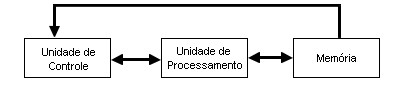
\includegraphics{Images/SISD.jpg}
    \caption{Classe SISD da Taxonomia de Flynn}\label{fig:sisd}
\end{figure}

\textbf{\simd:} Uma única instrução é responsável pelo processamento de vários dados. Define o funcionamento de processadores vetoriais e matriciais. Diversos módulos de memória são necessários, as instruções seguem organizadas sequencialmente e possui uma unidade de controle e várias unidades de processamento. A Figura~\ref{fig:simd} ilustra essa classe.

\begin{figure}[t]
    \centering
    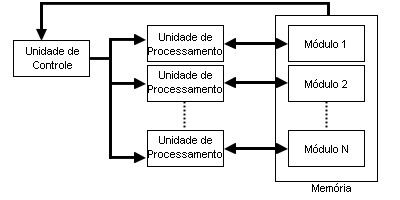
\includegraphics{Images/SIMD.jpg}
    \caption{Classe SIMD da Taxonomia de Flynn}\label{fig:simd}
\end{figure}

\textbf{\misd:} Múltiplas instruções trabalhando no mesmo fluxo de dados. Esta classe da Taxonomia de Flynn é impossível de ser colocada em prática. A Figura~\ref{fig:misd} ilustra essa classe.

\begin{figure}[t]
    \centering
    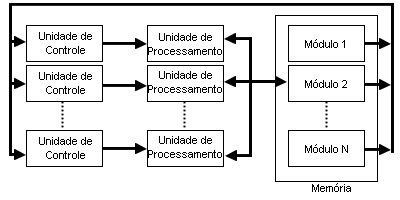
\includegraphics{Images/MISD.jpg}
    \caption{Classe MISD da Taxonomia de Flynn}\label{fig:misd}
\end{figure}

\textbf{\mimd:} Múltiplas instruções trabalhando em múltiplos dados. Possui várias unidades de controle, várias unidades de processamento e vários módulos de memória. Qualquer grupo de máquinas operando em conjunto, com interação entre elas, pode ser classificado como \mimd. A Figura~\ref{fig:mimd} ilustra essa classe.

\begin{figure}[t]
    \centering
    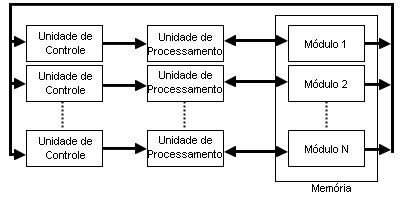
\includegraphics{Images/MIMD.jpg}
    \caption{Classe MIMD da Taxonomia de Flynn}\label{fig:mimd}
\end{figure}

Além da Taxonomia de Flynn, as arquiteturas paralelas podem ser classificadas segundo o compartilhamento de memória. Multiprocessadores trabalham com vários processadores podendo acessar a mesma memória compartilhada, enquanto nos multicomputadores cada processador possui sua própria memória, fazendo necessário o uso de uma rede de interconexão para trocar informações.

\subsubsection{Multiprocessadores}

Multiprocessadores são sistemas nos quais múltiplas \cpus compartilham acesso à mesma memória. Uma propriedade que forma a base da comunicação entre processadores é: uma \cpu escreve algum dado na memória e outra lê o mesmo dado. Sistemas multiprocessadores possuem algumas características únicas, como sincronização de processos e escalonamento, por exemplo. A Figura~\ref{fig:mproc} exibe graficamente a arquitetura de um multiprocessador.

\begin{figure}[t]
    \centering
    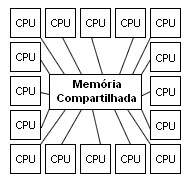
\includegraphics{Images/Multiprocessador.jpg}
    \caption{Multiprocessador}\label{fig:mproc}
\end{figure}

Alguns multiprocessadores possuem a característica de que uma certa palavra de memória possa ser lida na mesma velocidade que qualquer outra palavra. Essas máquinas são chamadas de \uma. Máquinas que não apresentam essa propriedade são chamadas de \numa \cite{Tanenbaum2015}.

\subsubsection{Multicomputadores}

Multicomputadores são sistemas nos quais cada \cpu possui sua própria memória, não podendo ser diretamente acessada por nenhum outro processador. A troca de informações nesse sistema é feita através de uma rede de interconexão. A Figura~\ref{fig:mcomp} exibe graficamente a arquitetura de um multicomputador.

\begin{figure}[t]
    \centering
    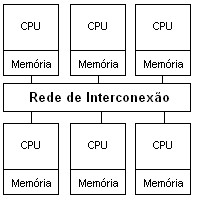
\includegraphics{Images/Multicomputador.jpg}
    \caption{Multicomputador}\label{fig:mcomp}
\end{figure}

O acesso à memória nos multicomputadores é classificado como \norma, afinal não é possível que uma \cpu tenha acesso à memória remota \cite{Hwang1998}.

\subsubsection{Aceleradores}

Uma \gpgpu, ou um acelerador, é uma placa gráfica que pode ser usada para computação de propósito geral. São classificados como \simd pela Taxonomia de Flynn, permitindo que vários dados possam ser processados em paralelo. As placas atuais utilizam uma extensão desse conceito, chamada de \simt, garantindo a execução da mesma instrução em threads diferentes. A Figura~\ref{fig:acel} exibe graficamente a arquitetura de um acelerador.

\begin{figure}[t]
    \centering
    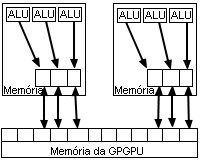
\includegraphics{Images/gpgpu.jpg}
    \caption{Acelerador}\label{fig:acel}
\end{figure}

\gpgpus são compostas por vários processadores, que possuem vários núcleos cada, sendo que cada processador possui sua própria memória interna, compartilhada pelas suas \alus, e uma memória compartilhada entre todos os processadores \cite{Miranda2010}.

\subsection{Programação Paralela}

A seguir serão apresentados os principais meios de desenvolvimento de aplicações paralelas para multiprocessadores, multicomputadores e aceleradores.

\subsubsection{Programação para Multiprocessadores}

A principal \api de desenvolvimento de aplicações paralelas para multiprocessadores é o \openMP. O \openMP é baseado em diretivas de compilação, podendo ser usado em C/C++ ou em Fortran, combinando regiões sequenciais e paralelas no mesmo código fonte. As diretivas permitem a criação de regiões paralelas nas quais múltiplas threads são criadas e executadas em paralelo. O número de threads em uma região paralela pode ser determinado pelo usuário. Todavia, em programas paralelos utiliza-se normalmente uma thread para cada núcleo de processamento da arquitetura.

Para C/C++ as diretivas são da seguinte maneira:
\begin{center}
\texttt{\#pragma omp [diretiva] [atributos]}
\end{center}

A Figura~\ref{fig:lstopenmp} exemplifica a soma de dois vetores utilizando o \openMP. Neste exemplo, a diretiva \texttt{parallel} foi usada para iniciar uma região paralela, enquanto a diretiva \texttt{for} serviu para paralelizar o laço, dividindo a execução das iterações do mesmo em várias \textit{threads}. Foram declarados 3 vetores, e depois os vetores \texttt{a} e \texttt{b} foram somados e o resultado da soma foi armazenado no vetor \texttt{c}.

Variáveis globais são compartilhadas entre as threads, porém variáveis criadas dentro de um laço são privadas. O sucesso do \openMP se deve ao fato de que ele é bem simples de ser usado e, por conta de uma alta aceitação, consegue ser executado em várias plataformas diferentes \cite{Chapman2008}.

\subsubsection{Programação para Multicomputadores}

A principal \api de desenvolvimento de aplicações paralelas para multicomputadores é o \mpi. O \mpi permite que dados sejam transmitidos entre processos em um ambiente de memória distribuída. As principais características do \mpi são portabilidade do código fonte, implementação eficiente, várias funcionalidades e suporte à arquiteturas paralelas heterogêneas.

\begin{figure}[t]
    \centering
    \begin{lstlisting}
    int main(int argc, char *argv[]) {
        int a[1000], b[1000], c[1000];
    
        initialize_vectors(&a, &b);
    
        #pragma omp parallel for
        for (int i = 0; i < 1000; i++)
            c[i] = a[i] + b[i];
                
        return 0;
    }
    \end{lstlisting}
    \caption{Exemplo da soma de vetores em OpenMP.}
    \label{fig:lstopenmp}
\end{figure}

Programas escritos em Fortran ou C/C++ são compilados normalmente, porém ligados com a biblioteca \mpi. O \mpi fornece funções do tipo \texttt{send} e \texttt{receive} síncronas e assíncronas para fazer a comunicação entre os processos. Além disso, ele oferece funções específicas e otimizadas para comunicação em grupo. Basicamente, as funções de envio e recebimento recebem como entrada os dados a serem transmitidos (assim como seu tipo e a quantidade de dados), o destinatário/remetente, entre outras.

A Figura~\ref{fig:lstmpi} exemplifica a soma de dois vetores utilizando o \mpi. Nas linhas 2 a 3 é feita a declaração das variáveis necessárias, no caso os vetores \texttt{a}, \texttt{b}, \texttt{c} e duas variáveis de controle que serão inicializadas pelo MPI (linhas 7 a 8) e conterão o \textit{rank} do processo \mpi (\texttt{rank}) e a quantidade total de processos \mpi (\texttt{size}). O ambiente paralelo do \mpi é inicializado na linha 4. A linha 11 é somente executada pelo processo \mpi cujo \textit{rank} é igual à 0 e servirá para inicializar os vetores. As linhas 13 e 14 calculam a quantidade de elementos que cada processo irá receber. As linhas 16 a 19 usam o \texttt{Scatter}, que é uma função do \mpi que divide o vetor em partes iguais, no caso com a quantidade de elementos calculada anteriormente, e envia cada uma dessas partes para um processo diferente. As linhas 21 a 23 somam os vetores divididos e salvam o resultado num vetor temporário. Cada processo terá seu próprio resultado, independente dos outros processos. Nas linhas 25 e 26 é utilizada a função \texttt{Allgather}, que faz cada processo enviar sua parte do resultado calculado para todos os outros processos, juntando todas as partes e formando o vetor completo que contém o resultado final da soma, no caso o vetor \texttt{c}. A linha 28, por fim, encerra o ambiente paralelo do \mpi.

O \mpi não é uma implementação, mas sim uma especificação, possuindo diversas implementações diferentes. Uma das mais utilizadas implementações que existem atualmente é o OpenMPI, uma biblioteca de código aberto que implementa o \mpi \cite{Gropp1999}.

\begin{figure}[t]
    \centering
    \begin{lstlisting}
    int main(int argc, char *argv[]) {
        int a[1000], b[1000], c[1000];
        int rank, size;
        
        MPI_Init(&argc, &argv);
        
        MPI_Comm_rank(MPI_COMM_WORLD, &rank);
        MPI_Comm_size(MPI_COMM_WORLD, &size);
        
        if(rank == 0)
            initialize_vectors(&a, &b);
        
        int elements_per_proc = 1000 / size;
        int sub_a[elements_per_proc], sub_b[elements_per_proc];
    
        MPI_Scatter(a, elements_per_proc, MPI_INT, &sub_a,
                    elements_per_proc, MPI_INT, 0, MPI_COMM_WORLD);
        MPI_Scatter(b, elements_per_proc, MPI_INT, &sub_b,
                    elements_per_proc, MPI_INT, 0, MPI_COMM_WORLD);
    
        int temp[elements_per_proc];
        for (i = 0; i < elements_per_proc; i++)
            temp[i] = sub_a[i] + sub_b[i];
        
        MPI_Allgather(&temp, elements_per_proc, MPI_INT,
                   c, elements_per_proc, MPI_INT, MPI_COMM_WORLD);
        
        MPI_Finalize();
        
        return 0;
    }
    \end{lstlisting}
    \caption{Exemplo da soma de vetores em MPI}
    \label{fig:lstmpi}
\end{figure}

\subsubsection{Programação para Aceleradores}

A principal \api de desenvolvimento para aceleradores é o \cuda, tecnologia da NVIDIA. A ideia é que os desenvolvedores possam usar o processamento da \gpu para computação de propósito geral. A palavra chave \texttt{global} mostra para o compilador que a função a seguir será executada na \gpu. O \cuda também oferece funções para alocar dinamicamente dados na memória da \gpu, podendo alocar com a função \texttt{cudaMalloc()} e depois liberar com a função \texttt{cudaFree()} \cite{Sanders2010}.

A Figura~\ref{fig:lstcuda} exemplifica a soma de dois vetores, vistos anteriormente em \openMP e \mpi, porém utilizando a tecnologia \cuda. As linhas 1 a 5 utilizam o prefixo \texttt{global}, cujo objetivo é informar que o código da função será executado na \gpu. A função \texttt{add} é chamada da seguinte forma: \texttt{$add\lll N,1 \ggg$}, onde o parâmetro \texttt{N} é o número de blocos que serão criados pela \gpu para executar em paralelo. A variável \texttt{blockIdx.x} informa qual bloco está sendo executado. O código \texttt{if (tid < 1000)} garante que não haverá acesso ao lixo de memória, no caso de existir mais blocos de \gpu do que elementos para serem calculados. As linhas 8 e 9 declaram os vetores e variáveis necessários. As linhas 11 a 13 são responsáveis por alocar a memória da \gpu utilizando a função \texttt{cudaMalloc()}. As linhas 17 a 20 copiam os vetores \texttt{a} e \texttt{b} para a \gpu. A linha 22 chama a função \texttt{add} que será executada na placa gráfica. As linhas 24 e 25 copiam o vetor \texttt{c} de volta para a \cpu. As linhas 27 a 29 liberam a memória alocada na \gpu usando a função \texttt{cudaFree()} e finalizam a execução do programa.

\begin{figure}[t]
    \centering
    \begin{lstlisting}
    __global__ void add(int *a, int *b, int *c) {
        int tid = blockIdx.x;
        if (tid < 1000)
            c[tid] = a[tid] + b[tid];
    }
    
    int main( void ) {
        int a[1000], b[1000], c[1000];
        int *dev_a, *dev_b, *dev_c;
        
        HANDLE_ERROR(cudaMalloc((void**)&dev_a, 1000 * sizeof(int)));
        HANDLE_ERROR(cudaMalloc((void**)&dev_b, 1000 * sizeof(int)));
        HANDLE_ERROR(cudaMalloc((void**)&dev_c, 1000 * sizeof(int)));
        
        initialize_vectors(&a, &b);
        
        HANDLE_ERROR(cudaMemcpy(dev_a, a, 1000 * sizeof(int),
                                cudaMemcpyHostToDevice));
        HANDLE_ERROR(cudaMemcpy(dev_b, b, 1000 * sizeof(int),
                                cudaMemcpyHostToDevice));
                                
        add<<<1000,1>>>(dev_a, dev_b, dev_c);
        
        HANDLE_ERROR(cudaMemcpy(c, dev_c, 1000 * sizeof(int),
                                cudaMemcpyDeviceToHost));
                                
        cudaFree(dev_a);
        cudaFree(dev_b);
        cudaFree(dev_c);
        
        return 0;
    }
    \end{lstlisting}

    \caption{Exemplo da soma de vetores em CUDA}
    \label{fig:lstcuda}
\end{figure}

Para compilar o código usando o compilador CUDA C++ basta executar:
\begin{center}
\texttt{nvcc add.cu -o add\_cuda}
\end{center}

\section{Criptografia de Dados}

Do grego \textit{Kriptos} (oculto) e \textit{Grapho} (escrita), é o nome dado à ciência de codificar e decodificar mensagens. Tem como meta garantir:
\begin{itemize}
    \item \textbf{Autenticação}: Identificar o remetente da mensagem;
    \item \textbf{Integridade}: Não adulteração da mensagem original;
    \item \textbf{Não Recusa}: Remetente não pode negar que enviou a mensagem.
\end{itemize}

A criptografia pode ser classificada como simétrica ou assimétrica, dependendo de como as chaves de codificação e decodificação são utilizadas. Há também o resumo criptográfico, ou Hash, que é um número pequeno que representa todo um documento \cite{Stallings2014}.

\subsection{Criptografia Simétrica}

O conceito mais antigo de criptografia é chamado de criptografia simétrica. Neste modelo a chave que dá acesso à mensagem é a mesma, tanto para codificar como para decodificar a mensagem, e deve permanecer em segredo, por isso é chamada de chave privada. A chave é utilizada para evitar que terceiros tenham acesso à mensagem, mesmo conhecendo o algoritmo utilizado e tendo em mãos a mensagem cifrada. A Figura~\ref{fig:cripsim} exibe o funcionamento da criptografia simétrica.

A maior vantagem da criptografia simétrica é sua facilidade de uso e velocidade para executar os algoritmos criptográficos. O problema deste modelo é que a chave usada para cifrar precisa ser compartilhada com o destinatário, abrindo uma brecha para terceiros interceptarem a chave \cite{Stallings2014}.

\begin{figure}[t]
    \centering
    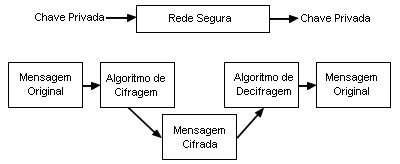
\includegraphics{Images/Simetrica.jpg}
    \caption{Criptografia Simétrica}\label{fig:cripsim}
\end{figure}

Os principais algoritmos de criptografia simétrica são:
\begin{itemize}
    \item \aes: Desenvolvido pelo \textit{National Institute of Standards and Technology}, é o algoritmo padrão usado pelo governo dos Estados Unidos da América. Possui um tamanho de bloco fixo em 128 bits, chave de 128, 192 ou 256 bits, rápido e fácil de executar e utiliza pouca memória.
    \item \des: Desenvolvido pela IBM em 1977, foi o algoritmo mais utilizado no mundo até a padronização do \aes. Possui um tamanho de chave pequeno, de apenas 56 bits, o que possibilita quebrar o algoritmo por força bruta. A partir de 1993 passou a ser recomendada a utilização do 3DES, uma variação do \des no qual o ciframento é feito 3 vezes seguidas, porém é muito lento para se tornar um algoritmo padrão.
\end{itemize}

\subsection{Criptografia Assimétrica}

Modelo desenvolvido pelo matemático Clifford Cocks, no qual as chaves para cifrar e decifrar são diferentes, chamadas de assimétricas. A chave pública pode ser vista por qualquer pessoa, porém a chave privada permanece em posse apenas do titular. Uma pessoa pode utilizar sua chave privada para decodificar uma mensagem criptografada com sua chave pública. A Figura~\ref{fig:cripasim} exibe o funcionamento da criptografia assimétrica.

A maior vantagem deste modelo é a segurança, uma vez que a chave privada não é compartilhada. Porém a velocidade é muito menor do que os algoritmos simétricos, o que pode não permitir o seu uso em algumas situações \cite{Stallings2014}.

\begin{figure}[t]
    \centering
    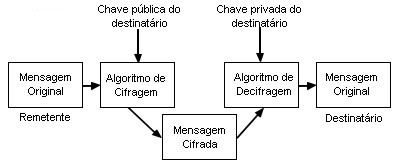
\includegraphics{Images/Assimetrica.jpg}
    \caption{Criptografia Assimétrica}\label{fig:cripasim}
\end{figure}

Os principais algoritmos de criptografia assimétrica são:
\begin{itemize}
    \item \rsa: Desenvolvido em 1977 no \mitt. É o algoritmo assimétrico mais utilizado no momento, além de ser um dos mais poderosos que existem. É baseado no fato de que dois números primos são facilmente multiplicados para gerar um terceiro número, porém é muito difícil recuperar esses números a partir do terceiro número. Para se descobrir a chave privada, é necessário fatorar números muito grandes, o que pode levar um tempo considerável. Assim, a segurança do RSA é baseada na dificuldade de fatoração de números primos grandes.
    \item \elgamal: Baseado em grandes cálculos matemáticos. Sua segurança é baseada na dificuldade de calcular logaritmos discretos em um corpo finito.
    \item \dhes: Mais antigo dos métodos assimétricos, também é baseado no problema dos logaritmos discretos. Não é possível usá-lo para assinaturas digitais.
\end{itemize}

\subsection{Resumo Criptográfico}

Resumo criptográfico, também conhecido por hash, são funções criptográficas unidirecionais, ou seja, não é possível obter o conteúdo original a partir do hash. Uma característica dessas funções é que, independente do tamanho do texto, hash sempre terá um tamanho fixo, geralmente de 128 bits. Outra propriedade é que duas mensagens distintas não irão gerar o mesmo hash \cite{Pfleeger2015}.

Os principais algoritmos de hash utilizados atualmente são:
\begin{itemize}
    \item \mdd: Desenvolvido por Ron Rivest, do \mitt. Produz um hash de 128 bits. É um algoritmo rápido, simples e seguro, porém não é recomendado devido ao pequeno tamanho de 128 bits, sendo preferível um hash de maior valor.
    \item \sha: Criado pela \nsa, gera um hash de 160 bits. É recomendável o uso do \sha-2, uma variação mais forte e segura do que o \sha-1, devido ao maior número de bits que é gerado.
\end{itemize}

Alguns usos de funções de hash são:

\begin{itemize}
    \item \textbf{Verificar integridade de arquivos}: Basta tirar o hash de um arquivo e guardá-lo. Em um momento futuro é possível tirar o hash novamente e comparar com o antigo, se forem iguais então o arquivo está íntegro.
    \item \textbf{Armazenamento de senhas}: A forma mais segura de armazenar uma senha é armazenar o hash da mesma, afinal não é possível obter a senha original. Quando precisar ser feita a verificação se uma senha digitada está correta, basta comparar o hash da senha digitada com o hash armazenado, se forem iguais então a senha está correta.
\end{itemize}

\section{Compressão de Dados}

Comprimir dados é o ato de reduzir o tamanho de arquivos, diminuindo o espaço que eles ocupam em disco e aumentando o desempenho de aplicativos que usam esses dados. Essa técnica é interessante para diversos fins, desde um usuário de smartphone que deseja armazenar mais fotos no seu aparelho até um serviço \textit{web} que envia muitos dados através da internet. A Figura~\ref{fig:compression} mostra o conceito da compressão de dados.

Existem duas formas de compressão, com perdas e sem perdas, que descartam partes insignificantes do arquivo ou mantém todo o conteúdo, respectivamente.

\begin{figure}[t]
    \centering
    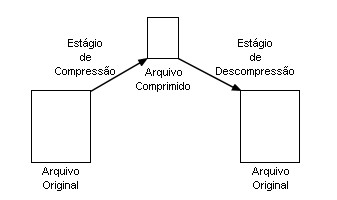
\includegraphics{Images/Compressao.jpg}
    \caption{Compressão de Dados}\label{fig:compression}
\end{figure}

\subsection{Compressão sem Perdas}

A compressão sem perdas, ou \textit{Lossless Data Compression}, garante que os dados obtidos após a descompressão serão exatamente iguais aos dados originais que foram comprimidos. Essa técnica é geralmente utilizada quando não se pode perder nada do conteúdo original, como arquivos de texto ou informações delicadas de experimentos científicos por exemplo.

\subsection{Compressão com Perdas}

A compressão com perdas, ou \textit{Lossy Data Compression}, garante que os dados obtidos após a descompressão serão bastante parecidos com o conteúdo original, com diferenças mínimas. Essa técnica é geralmente utilizada para arquivos de áudio ou vídeo, nos quais a diferença de conteúdo é imperceptível e o tamanho é reduzido consideravelmente.

\subsection{Compressão de Textos}

A compressão de textos se baseia em representar o texto original de outra maneira, usando símbolos que ocupem menos espaço. Com isso se ganha também velocidade ao se fazer busca em grandes documentos. A desvantagem é o tempo necessário para a descompressão do conteúdo.

Um dos métodos mais conhecidos é o método de Huffman, de 1952. Nele, um código único é associado a cada caractere diferente do texto. Códigos menores são associados com os caracteres que aparecem com maior frequência. É o método mais eficiente para compressão de textos em linguagem natural, com 60\% de redução no tamanho do arquivo. O método de Huffman elimina todos os espaços entre palavras. No momento da descompressão, a não ser que exista um separador, como uma vírgula, um espaço é inserido entre as palavras \cite{Salomon2007}.

\subsection{Compressão de Imagens}

Existem formatos de imagens que comprimem com ou sem perdas. Os mais conhecidos formatos de compressão sem perdas são \png, \jpegg e \tiff.

A compressão sem perdas explora a redundância entre pixeis e garante que nenhum dado será perdido. É especialmente importante em casos nos quais a fidelidade dos dados é muito importante, como para a fotografia profissional. Os algoritmos mais usados são o \rle, \lz, \lzw e o algoritmo de Huffman, o qual é usado nos formatos \png e \tiff.


Dentre os métodos com perdas, os mais conhecidos são \jpeg e \gif. A compressão com perdas busca eliminar detalhes que não são perceptíveis ao olho humano. Porém há formatos, como o \gif, que utilizam um grau maior de perda, causando uma degradação grande na imagem.

%\subsubsection{A Transformada DCT}
%
%A transformada discreta do cosseno é similar à transformada de Fourier, porém utiliza apenas números reais. É esperado que os pixeis de uma imagem tenham uma transição contínua de um para outro. A \dct consiste em encontrar uma base na qual os primeiros elementos terão pouca variação, e os últimos terão grande variação. Assim, podemos escrever os pixeis da imagem como uma combinação linear da base, na qual os últimos coeficientes são praticamente nulos, podendo ser eliminados.
%
%Como uma imagem é representada como uma matriz de pixeis, é utilizada a \dct bidimensional, no qual a transformada é aplicada primeiramente nas linhas e depois nas colunas. A equação da transformada para uma imagem \textit{P} de tamanho \textit{n X n} é dada pela seguinte equação \cite{ahmed1974}:
%
%\begin{equation}
%    Gij=\frac{1}{\sqrt{2n}}CiCj\sum_{x=0}^{n-1}\sum_{y=o}^{n-1} Pxy \;  \cos\bigg(\frac{(2y+1)j\pi}{2n}\bigg) \;  %\cos\bigg(\frac{(2x+1)i\pi}{2n}\bigg)
%\end{equation}
%para $$0 \leqslant i, j \leqslant n-1$$
%onde $$Cf=\frac{1}{\sqrt{2}}, f=0\quad ou \quad Cf=1,f>0$$
%
%A recuperação dos dados originais é feita através da transformação inversa, conhecida por \idct bidimensional:
%
%\begin{equation}
%    Pxy=\frac{1}{4}\sum_{i=0}^{n-1}\sum_{j=0}^{n-1}CiCjCij \;
%    \cos\bigg(\frac{(2x+1)i\pi}{2n}\bigg) \;
%    \cos\bigg(\frac{(2y+1)j\pi}{2n}\bigg)
%\end{equation}
%
%\todo[inline]{Aqui vale um comentário. A fórmula é bonita, mas sabes explicá-la? Simplesmente colocar uma fórmula no texto e não saber explicá-la não faz muito sentido. Nesse caso, aqui precisa ser adicionado um texto para explicar as duas equações apresentadas anteriormente.}
\chapter{O Algoritmo de Cripto-Compressão GMPR}
\label{cap3}

O algoritmo de cripto-compressão \gmpr foi desenvolvido pela \textit{Sheffield Hallam University} em MATLAB~\cite{shu13715}. Neste projeto de trabalho de conclusão de curso, este algoritmo será reescrito em C++ para que seja possível paralelizá-lo.

O algoritmo \gmpr foi desenvolvido com o foco em imagens, sendo superior em qualidade em relação ao conhecido formato \jpeg e com qualidade equivalente ao formato \jpegg. A Tabela~\ref{tab:gmprjpeg} mostra uma comparação do algoritmo \gmpr com os formatos \jpeg e \bmp para imagens 3D.

Ele utiliza a \dct e um algoritmo de minimização de matrizes no estágio de compressão, além de um novo método concorrente de busca binária no estágio de descompressão. Os principais passos do algoritmo de compressão consistem em dividir a imagem em blocos e aplicar a \dct para cada bloco, aplicar o algoritmo de minimização de matrizes nos coeficientes \texttt{AC} de cada bloco, reduzindo a matriz para 1/3 do tamanho, construir uma \lut para permitir a recuperação dos dados originais no estágio de descompressão, aplicar um delta na lista de coeficientes \texttt{DC} e aplicar a codificação aritmética nos resultados. O estágio de descompressão utiliza a \lut e o algoritmo de busca binária para recuperar todos os coeficientes \texttt{AC}, enquanto os coeficientes \texttt{DC} são recuperados revertendo a codificação aritmética, e, finalmente, a \dct inversa recupera a imagem original \cite{shu13715}. A Figura~\ref{fig:gmprcompression} ilustra o processo de compressão.

\begin{table}[t]
\centering
    \begin{tabular}{| l | l | l | l |}
    \hline
        Imagem & \bmp & \jpeg & \gmpr \\ \hline
        Maçã & 336 MB & 52.4 MB & 0.929 MB \\ \hline
        Estátua & 366 MB & 58.5 MB & 0.916 MB \\ \hline
        Rosto & 200.7 MB & 45.5 MB & 0.784 MB \\ \hline
    \end{tabular}
    \caption{Compressão de Imagens 3D.}\label{tab:gmprjpeg}
\end{table}


\section{Compressão}

Primeiramente a imagem é dividida em blocos de tamanho \texttt{n}, e então é aplicada a \dct em cada bloco. Cada bloco consiste de coeficientes \texttt{DC}, que são o valor médio do bloco, e os demais coeficientes, chamados \texttt{AC}. A \dct, um processo sem perdas e reversível, serve para identificar redundâncias na imagem, ou seja, pixeis muito semelhantes em relação aos seus vizinhos.

Em seguida é aplicado o algoritmo de minimização de matrizes na lista de coeficientes \texttt{AC}, eliminando todos os zeros, que geralmente são muitos, reduzindo seu tamanho e produzindo o vetor minimizado. São definidas 3 chaves que irão multiplicar cada 3 entradas deste vetor minimizado, e então os 3 valores são somados, ou seja, cada 3 valores do vetor é transformado em apenas 1, reduzindo o tamanho para 1/3 do original, produzindo o vetor minimizado codificado.

A etapa de descompressão inicia na recuperação dos coeficientes \texttt{DC}, revertendo a codificação aritmética. Os coeficientes \texttt{AC} são recuperados através da busca binária, utilizando as 3 chaves geradas na compressão é possível recuperar o vetor minimizado, decodificando-o.

Em seguida os coeficientes \texttt{DC} a \texttt{AC} são combinados, recolocando todos os zeros que foram removidos na compressão, e em seguida aplicando a \dct inversa para recuperar a imagem original \cite{shu13715}.

\section{Criptografia}

De modo geral, o algoritmo \gmpr inicia a etapa de cifragem obtendo o texto plano e convertendo-o para \texttt{ASCII}. Em seguida é obtida uma lista dos caracteres contidos no arquivo, sem repetir nenhum. Por exemplo: o texto ``abac'' irá gerar uma lista contendo os caracteres ``abc'', não incluindo o caractere ``a'' duas vezes.

\begin{figure}[t]
    \centering
    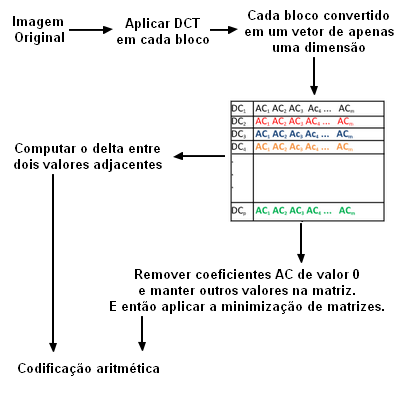
\includegraphics{Images/GMPRCompression.png}
    \caption{Estágio de Compressão do GMPR}
    \label{fig:gmprcompression}
\end{figure}

São geradas 3 chaves aleatórias. A partir disso é gerada uma lista chamada \texttt{nCoded}, na qual a cada 3 caracteres do texto é gerado 1 elemento codificado usando as chaves geradas. O texto ``abac'' geraria 2 elementos nessa lista, pois ``aba'' seria codificado no primeiro elemento e ``c'' codificado no segundo elemento;

É criado um vetor chamado \texttt{codedvector} que é formado pelas 3 chaves, pela lista única de caracteres e pela lista \texttt{nCoded}. Em seguida o texto final codificado é gerado.

\begin{figure}[t]
    \centering
    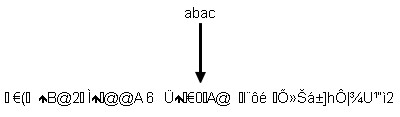
\includegraphics{Images/CifraGMPR.jpg}
    \caption{Binário gerado pelo algoritmo GMPR}\label{fig:gmpr}
\end{figure}

Para decifrar o conteúdo e obter o arquivo original, o algoritmo começa obtendo o texto cifrado e transformando-o em um vetor. Em seguida são extraídas as 3 chaves usadas no processo de cifragem, a lista única de caracteres e a lista \texttt{nCoded}. Por fim, o conteúdo é decodificado.

Se o arquivo cifrado com o algoritmo \gmpr for aberto em algum editor de texto será mostrado algo parecido com o exemplo da Figura~\ref{fig:gmpr}. As seções a seguir apresentam os pseudo-códigos das etapas de cifragem e decifragem do algoritmo.

\subsection{Algoritmo de Cifragem}
		
\begin{algorithm}[t]
\begin{algorithmic}[1]
\footnotesize
    \vspace{0.2em}
    \State $nData \gets$ \Call{abrirArquivoOriginal}{}
    \vspace{0.5em}
    \For{$i$ \textbf{from} $0$ \textbf{to} $nData.tamanho()$}
    \vspace{0.2em}
        \If{$!(nLimited \supset nData[i])$}
            \vspace{0.2em}
            \State \Call{adicionarElemento}{$nLimited$, $nData[i]$}
        \EndIf
    \EndFor
    \vspace{0.5em}
    \State $K[0] \gets$ \Call{rand}{} \% 1001
    \State $K[1] \gets$ (\Call{rand}{} \% 11) * 2 * $maxvalue$
    \State $K[2] \gets$ $K[1]$ * $maxvalue$ * (\Call{rand}{} \% 11)
    \vspace{0.5em}
    \While{$i$ <= $nData.tamanho()$}
        \vspace{0.2em}
        \State $nCoded[i] \gets K[0]*nData[i] + K[1]*nData[i+1] + K[2]*nData[i+2]$
        \State $i \gets i + 3$
    \EndWhile
    \vspace{0.5em}
    \State \Call{adicionarElemento}{$codedvector$, $K$}
    \State \Call{adicionarElemento}{$codedvector$, $nLimited.tamanho()$}
    \State \Call{adicionarElemento}{$codedvector$, $nCoded.tamanho()$}
    \State \Call{adicionarElemento}{$codedvector$, $nLimited$}
    \State \Call{adicionarElemento}{$codedvector$, $nCoded$}
    \vspace{0.5em}
    \State string $msg \gets$ \Call{paraString}{$codedvector$}
    \vspace{0.5em}
    \State $stats \gets$ \Call{obterListaIntervaloProbabilidades}{}
    \For{$i$ \textbf{from} $0$ \textbf{to} $nData.tamanho()$}
        \vspace{0.2em}
        \State \Call{AplicaProbabilidades}{$nData[i]$, $stats$}
    \EndFor
    \vspace{0.5em}
    \State \Call{EscreverDisco}{$stats$}
\end{algorithmic}
\caption{Cifragem}
\label{algorithm: gmprc}
\end{algorithm}

Nas linhas 2 a 4 é criada e preenchida a \texttt{nLimited}, uma lista contendo todos os caracteres únicos do texto plano. 

Em seguida as 3 chaves aleatórias são geradas nas linhas 5 a 7. \texttt{K[0]} é gerada entre 0 e 1000. \texttt{K[1]} gera um valor entre 0 e 10 e depois multiplica pelo dobro do maior caractere do texto plano. \texttt{K[2]} gera um valor entre 0 e 10, multiplica pela chave \texttt{K[1]} e depois multiplica pelo maior caractere do texto plano.

Nas linhas 8 a 10 é criada e preenchida a \texttt{nCoded}, uma lista que contém as chaves \texttt{K} multiplicadas pelo texto plano. Nas linhas 11 a 15 é criado e preenchido o \texttt{codedvector}, um vetor que contém as chaves \texttt{K}, o tamanho da lista \texttt{nLimited}, o tamanho da lista \texttt{nCoded}, o conteúdo da lista \texttt{nLimited} e o conteúdo da lista \texttt{nCoded}.

Na linha 16 é convertido o vetor \texttt{codedvector} para \texttt{string}.

Na linha 17 é obtida uma lista de intervalos de probabilidades para cada símbolo do texto plano. Em seguida são aplicados os intervalos à cada elemento do texto e adicionados ao texto final codificado nas linhas 18 e 19. Por fim o arquivo é salvo em disco na linha 20.

\subsection{Algoritmo de Decifragem}

\begin{algorithm}[t]
\begin{algorithmic}[1]
\footnotesize
    \vspace{0.2em}
    \State $msg \gets$ \Call{ArDecodeFile}{}
    \vspace{0.5em}
    \State $data \gets$ \Call{paraVetor}{$msg$}
    \vspace{0.5em}
    \State $K[0] \gets data[0]$
    \State $K[1] \gets data[1]$
    \State $K[2] \gets data[2]$
    \vspace{0.5em}
    \State $nL \gets data[3]$
    \vspace{0.5em}
    \State $nC \gets data[4]$
    \vspace{0.5em}
    \For{$i$ \textbf{from} $5$ \textbf{to} $5+nL$}
        \vspace{0.2em}
        \State $nLimited[i] \gets data[i]$
    \EndFor
    \vspace{0.5em}
    \For{$i$ \textbf{from} $5+nL+1$ \textbf{to} $5+nL+1+nC$}
        \vspace{0.2em}
        \State $nCoded[i] \gets data[i]$
    \EndFor
    \vspace{0.5em}
    \State $ultimaPos \gets data.tamanho()$
    \For{$r$ \textbf{from} $0$ \textbf{to} $ultimaPos$}
        \vspace{0.2em}
        \For{$i$ \textbf{from} $0$ \textbf{to} $nL$}
            \vspace{0.2em}
            \For{$j$ \textbf{from} $0$ \textbf{to} $nL$}
                \vspace{0.2em}
                \For{$k$ \textbf{from} $0$ \textbf{to} $nL$}
                    \vspace{0.2em}
                    \If{$data[r] == K[0]*nLimited[i] + K[1]*nLimited[j] + K[2]*nLimited[k]$}
                        \vspace{0.2em}
                        \State $nDecoded[3*r+0] \gets nLimited[i]$
                        \State $nDecoded[3*r+1] \gets nLimited[j]$
                        \State $nDecoded[3*r+2] \gets nLimited[k]$
                    \EndIf
                \EndFor
            \EndFor
        \EndFor
    \EndFor
    \vspace{0.5em}
    \State \Call{EscreverDisco}{$nDecoded$}
\end{algorithmic}
\caption{Decifragem}
\label{algorithm: gmprd}
\end{algorithm}

Na linha 1 a rotina \texttt{ArDecodeFile} abre o arquivo cifrado, faz uma leitura do cabeçalho e gera a lista de probabilidades que será usada para decodificar o arquivo. Em seguida a \texttt{string} é convertida para vetor na linha 2.

Nas linhas 3 a 5 são obtidas as 3 chaves que foram usadas para cifrar. O tamanho da lista de caracteres únicos \texttt{nLimited} é obtido na linha 6 e seu conteúdo obtido nas linhas 8 e 9. O tamanho da lista \texttt{nCoded}, que contém as chaves \texttt{K} multiplicadas pelo texto plano, é obtido na linha 7 e seu conteúdo obtido nas linhas 10 e 11.

Nas linhas 12 a 20 o texto é decodificado, obtendo o conteúdo original. É feito o processo inverso da geração da lista \texttt{nCoded} no processo de cifragem, e quando o elemento codificado é encontrado então ele é salvo na lista \texttt{nDecoded}. Por fim o arquivo é salvo em disco.
\chapter{Proposta}
\label{cap4}

O algoritmo descrito no capítulo anterior possui várias possibilidades de ganho de desempenho. Todavia, para que isso seja possível, uma versão em C/C++ precisará ser desenvolvida.

Este trabalho de conclusão de curso possui três etapas principais. Na primeira etapa, será feita uma implementação em C++ do algoritmo de cripto-compressão \gmpr. Com base nesta solução proposta, na segunda etapa serão estudadas formas de paralelizar o código para obter-se um desempenho ainda melhor. As \apis \openMP, \mpi e/ou \cuda serão exploradas para implementar soluções paralelas e/ou distribuídas para este problema. Por fim, na terceira etapa, serão realizados experimentos para medir o desempenho das soluções paralelas propostas.

No presente momento, somente as etapas de cifragem/decifragem foram implementadas em C++. As etapas de compressão/descompressão serão implementadas ao longo do primeiro semestre de 2018. A versão atual do código em C++ está disponível no GitHub\footnote{\url{https://github.com/leandroperin/ParallelCryptoCompression}}.

A seguir, serão apresentadas algumas ideias iniciais de paralelização das etapas de cifragem/decifragem.

\section{Paralelismo com Multiprocessadores}

A primeira ideia de paralelização do código é a utilização do \openMP para executar as partes mais pesadas da aplicação em múltiplos núcleos do processador. Conforme visto no Capítulo~\ref{cap3}, o algoritmo possui muitos laços do tipo \texttt{for}, o que permite a utilização da biblioteca \openMP para executar esses laços em paralelo (através da diretiva \texttt{omp parallel for}), garantindo a correta execução das operações, porém em menos tempo.

Para isso, o objetivo inicial será definir em quais partes do código o programa leva mais tempo para executar, analisar se é possível quebrar essa parte em pedaços pequenos e atribuir múltiplas \texttt{threads} para a execução. Para isso, alguns experimentos preliminares foram feitos utilizando-se a ferramenta \texttt{Valgrind}\footnote{\url{http://valgrind.org/}} no Linux. A Figura~\ref{fig:valenc} apresenta os resultados obtidos para o algoritmo de codificação, enquanto a Figura~\ref{fig:valdec} apresenta os resultados para a decodificação.

\begin{figure}[t]
    \centering
    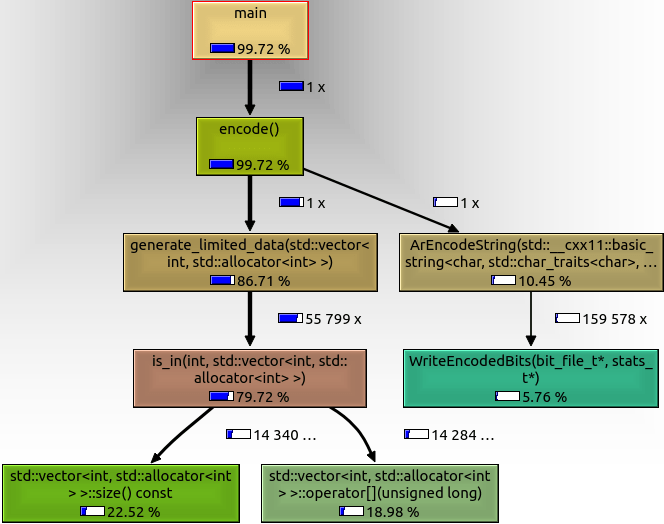
\includegraphics[width=8cm, height=6cm]{Images/ValgrindEncode.png}
    \caption{Resultados do Valgrind para a Codificação.}
    \label{fig:valenc}
\end{figure}

\begin{figure}[t]
    \centering
    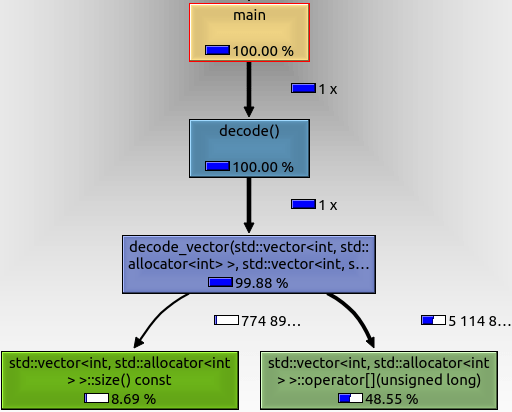
\includegraphics[width=8cm, height=6cm]{Images/ValgrindDecode.png}
    \caption{Resultados do Valgrind para a Decodificação.}
    \label{fig:valdec}
\end{figure}

Como é possível observar nas Figuras~\ref{fig:valenc} e~\ref{fig:valdec}, os métodos mais custosos em termos de tempo de execução são o \texttt{generate\_limited\_data()} para a parte de codificação, o qual utiliza o método \texttt{is\_in()} para verificar se algum caractere está presente na lista única de caracteres, e o \texttt{decode\_vector()} para a parte de decodificação, o qual usa o operador \texttt{[]} para acessar os elementos do vetor que contém os dados codificados.

O próximo passo é então fazer uso de regiões paralelas para dividir a computação executada nos métodos anteriormente citados a fim de melhorar o desempenho geral da solução. Após a definição das regiões paralelas, será necessário analisar se existem variáveis que serão compartilhadas entre as \textit{threads} e se há dependência entre elas. As cláusulas \texttt{shared} e \texttt{private} permitem descrever quais variáveis são compartilhadas entre todas as \textit{threads} e quais são privadas em cada \textit{thread}, respectivamente. Também, será verificada a existência de condições de corrida no código paralelizado. Nesses casos, regiões críticas do código, que são regiões que só podem ser executadas em uma \textit{thread} de cada vez, deverão ser protegidas com o uso da diretiva \texttt{omp critical}.

Por fim, será avaliada a possibilidade de uma solução híbrida com uso de \openMP e \mpi. Esta solução permitiria a execução da versão paralela da aplicação em \texttt{clusters}.

\section{Paralelismo com Aceleradores}

Tendo em  vista os resultados dos experimentos iniciais mostrados nas Figuras~\ref{fig:valenc} e~\ref{fig:valdec}, uma possibilidade seria a implementação de \textit{kernels} \cuda ou \opencl, uma solução de código aberto, para realizar a computação dos métodos mais custosos em \gpu. Neste caso, como mostrado no exemplo da Figura~\ref{fig:lstcuda}, será necessário implementar os \textit{kernels}, alocar memória na \gpu, copiar os dados que estão na \cpu e, por fim, liberar a memória utilizada.

As \gpus trabalham muito bem com operações matriciais, portanto uma possibilidade de melhora do código seria armazenar o conteúdo em matrizes e executar o algoritmo de cripto-compressão diretamente nas placas gráficas, garantindo um ganho de desempenho. \gpus possuem centenas de núcleos, e essa arquitetura massivamente paralela pode fazer o algoritmo \gmpr executar em um tempo consideravelmente menor.

Conteúdos que ganhariam bastante com o uso de \gpus são imagens e vídeos, afinal já são naturalmente armazenados em forma de matriz. A utilização do \cuda ou do \opencl seria bastante eficaz para esse tipo de conteúdo.

\section{Testes de Desempenho}

Após a implementação das soluções propostas (\openMP, \mpi e/ou \cuda/\opencl) serão feitos inúmeros testes e medições de desempenho, para que seja descoberta a melhor e mais rápida maneira de executar o algoritmo, garantindo o menor tempo de execução possível.
\chapter{Cronograma}
\label{cap5}

As atividades previstas no projeto estão descritas abaixo:

\begin{itemize}
    \item \textbf{A1: Estudo da fundamentação teórica.} Nesta etapa será feito o estudo de toda a fundamentação teórica do trabalho, seus conceitos e formas de colocá-los em prática.
    \item \textbf{A2: Produção do código sequencial.} Nesta etapa será refatorado todo o código do algoritmo, produzindo uma versão limpa e sequencial do mesmo.
    \item \textbf{A3: Elaboração da proposta.} Nesta etapa será elaborada a proposta do trabalho, incluindo os meios de paralelizar e melhorar o desempenho do algoritmo.
    \item \textbf{A4: Escrita do relatório do TCC I.} Nesta etapa será escrito o relatório do TCC I, que inclui a fundamentação teórica, descrição do algoritmo sequencial e proposta de paralelização. Entrega prevista para o mês de fevereiro.
    \item \textbf{A5: Implementação da proposta.} Nesta etapa serão implementadas as ideias propostas para a paralelização do algoritmo.
    \item \textbf{A6: Realização de experimentos.} Nesta etapa serão realizados experimentos com a versão paralela do código, fazendo medições de desempenho no mesmo.
    \item \textbf{A7: Escrita do rascunho do TCC II.} Nesta etapa será escrito o rascunho do TCC II, que inclui a proposta implementada e os resultados obtidos. Previsão de entrega para o mês de maio.
    \item \textbf{A8: Preparação da defesa pública.} Nesta etapa será elaborada a defesa pública do trabalho.
    \item \textbf{A9: Defesa pública.} Nesta etapa será realizada a defesa pública do trabalho desenvolvido. Data prevista para o mês de junho.
    \item \textbf{A10: Entrega da versão final do TCC II.} Nesta etapa serão feitas correções e ajustes solicitados no trabalho. Entrega da versão final prevista para o mês de julho.
\end{itemize}

A Figura~\ref{fig:cronograma} apresenta o cronograma previsto para a realização das atividades descritas anteriormente, o que inclui atividades durante o segundo semestre de 2017 e o primeiro semestre de 2018.

\begin{figure}
    \begin{center}
        \begin{ganttchart}[
        y unit title=0.4cm,
        y unit chart=0.6cm,
        hgrid,
        vgrid={{dotted, dotted, dotted, black}},
        title label font=\scriptsize,
        title/.append style={fill=gray!30},
        title height=1,
        bar/.append style={fill=gray!30,rounded corners=2pt},
        bar label font=\scriptsize,
        group label font=\scriptsize,
        ]{1}{20}
            \gantttitle{\textbf{2017}}{8}
            \gantttitle{\textbf{2018}}{12}\\
         	\gantttitle{\textbf{Ago}}{2}
         	\gantttitle{\textbf{Set}}{2}
        	\gantttitle{\textbf{Out}}{2}
        	\gantttitle{\textbf{Nov}}{2}
        	\gantttitle{\textbf{Fev}}{2}
        	\gantttitle{\textbf{Mar}}{2}
        	\gantttitle{\textbf{Abr}}{2}
        	\gantttitle{\textbf{Mai}}{2}
        	\gantttitle{\textbf{Jun}}{2}
        	\gantttitle{\textbf{Jul}}{2}\\
        	
        	\ganttbar{A1}{1}{2}\\
        	\ganttbar{A2}{3}{6}\\
            \ganttbar{A3}{7}{8}\\
            \ganttbar{A4}{8}{10}\\
            \ganttbar{A5}{11}{14}\\
            \ganttbar{A6}{13}{14}\\
            \ganttbar{A7}{14}{16}\\
            \ganttbar{A8}{17}{17}\\
            \ganttbar{A9}{18}{18}\\
            \ganttbar{A10}{19}{20}
        \end{ganttchart}
        \caption{Cronograma de Atividades}\label{fig:cronograma}
    \end{center}
\end{figure}
\chapter{Conclusão}
\label{cap6}

O algoritmo \gmpr funciona corretamente, cumprindo seu objetivo, porém apresenta um desempenho insatisfatório. Este trabalho busca analisar o código e melhorá-lo, garantindo que seu tempo de execução diminua e o torne possível de ser utilizado em alguma aplicação real.

A utilização das tecnologias \openMP, \mpi e/ou \cuda/\opencl aparentam ser as melhores opções disponíveis para melhorar o tempo de execução do algoritmo de cripto-compressão \gmpr. Elas serão implementadas e terão os resultados medidos, como forma de garantir os ganhos de desempenho.

Ter o algoritmo funcionando de forma eficiente é uma conquista muito interessante, pois o mesmo pode ser aplicado em serviços \textit{web} e na nuvem, reduzindo o armazenamento utilizado, os riscos de segurança e também o tempo necessário para enviar informações através da Internet.

O uso deste trabalho em projetos futuros é bastante possível, afinal esse algoritmo pode ser usado em qualquer projeto que tenha restrições de segurança das informações ou restrições de armazenamento. Há também a possibilidade desse projeto ser estendido para outras áreas, como a cripto-compressão de um banco de dados, dentre outras.
\chapter{Conclusão}
\label{cap7}

O algoritmo \gmpr funciona corretamente, cumprindo seu objetivo, porém apresenta um desempenho insatisfatório. Este trabalho busca analisar o código e melhorá-lo, garantindo que seu tempo de execução diminua e o torne possível de ser utilizado em alguma aplicação real.

A utilização das tecnologias \openMP, \mpi e/ou \cuda/\opencl aparentam ser as melhores opções disponíveis para melhorar o tempo de execução do algoritmo de cripto-compressão \gmpr. Elas serão implementadas e terão os resultados medidos, como forma de garantir os ganhos de desempenho.

Ter o algoritmo funcionando de forma eficiente é uma conquista muito interessante, pois o mesmo pode ser aplicado em serviços \textit{web} e na nuvem, reduzindo o armazenamento utilizado, os riscos de segurança e também o tempo necessário para enviar informações através da Internet.

O uso deste trabalho em projetos futuros é bastante possível, afinal esse algoritmo pode ser usado em qualquer projeto que tenha restrições de segurança das informações ou restrições de armazenamento. Há também a possibilidade desse projeto ser estendido para outras áreas, como a cripto-compressão de um banco de dados, dentre outras.

% ----------------------------------------------------------
% Finaliza a parte no bookmark do PDF
% para que se inicie o bookmark na raiz
% e adiciona espaço de parte no Sumário
% ----------------------------------------------------------
\phantompart

% ---
% Conclusão
% ---
%\chapter{Conclusão}
% ---

% ----------------------------------------------------------
% ELEMENTOS PÓS-TEXTUAIS
% ----------------------------------------------------------
\postextual
% ----------------------------------------------------------

% ----------------------------------------------------------
% Referências bibliográficas
% ----------------------------------------------------------
\bibliography{TCC.bib}

% ----------------------------------------------------------
% Glossário
% ----------------------------------------------------------
%
% Consulte o manual da classe abntex2 para orientações sobre o glossário.
%
%\glossary

%% ----------------------------------------------------------
% Apêndices
% ----------------------------------------------------------

% ---
% Inicia os apêndices
% ---
\begin{apendicesenv}

% Imprime uma página indicando o início dos apêndices
\partapendices

% ----------------------------------------------------------
\chapter{Quisque libero justo}
% ----------------------------------------------------------

\lipsum[50]

% ----------------------------------------------------------
\chapter{Nullam elementum urna vel imperdiet sodales elit ipsum pharetra ligula
ac pretium ante justo a nulla curabitur tristique arcu eu metus}
% ----------------------------------------------------------
\lipsum[55-57]

\end{apendicesenv}
% ---

%% ----------------------------------------------------------
% Anexos
% ----------------------------------------------------------

% ---
% Inicia os anexos
% ---
\begin{anexosenv}

% Imprime uma página indicando o início dos anexos
\partanexos

% ---
\chapter{Morbi ultrices rutrum lorem.}
% ---
\lipsum[30]

% ---
\chapter{Cras non urna sed feugiat cum sociis natoque penatibus et magnis dis
parturient montes nascetur ridiculus mus}
% ---

\lipsum[31]

% ---
\chapter{Fusce facilisis lacinia dui}
% ---

\lipsum[32]

\end{anexosenv}

%---------------------------------------------------------------------
% INDICE REMISSIVO
%---------------------------------------------------------------------
\phantompart
\printindex
%---------------------------------------------------------------------

\end{document}
